\documentclass[10pt, compress]{beamer}


\usepackage{booktabs}
\usepackage[scale=2]{ccicons}
\usepackage{url}
\usepackage{ drawstack }

\graphicspath{ {./pix/} }
\usetheme[useTitleProgressBar]{m}

\title{Radare2}
\subtitle{First r2babies steps - Long Version}
\author{Maxime Morin (@Maijin212)}
\date{\today}
\institute{BSides Las Vegas}

\begin{document}
\maketitle

\begin{frame}[fragile]
  \frametitle{About me}
    \begin{itemize}
    \item 22 y/o french expat @ Luxembourg
    \item Food, Travel and Languages <3
    \item I hate Bullshit
    \item Malware.lu CERT team leader (2days/week) and incident response @ European Commission CSIRC (3days/week)
    \item User of radare2 (impossibru!)
    \item I'm creating tests + documentation
    \end{itemize}
\end{frame}

\begin{frame}[fragile]
  \frametitle{Generality on radare2 framework}
  \begin{itemize}
  \item r1 2006, r2 2009
  \item Multi-(OSes|Archs|Bindings|FileFormats|...)
  \item 10 tools based on the framework
  \item Around 111 contributors from various fields
  \item GSOC + RSOC
  \item CLI/VisualMode/GUI/WebGUI
  \item around 350K LOC
  \end{itemize}
\end{frame}

\plain{Installation !}

\begin{frame}[fragile]
  \frametitle{Installation}
  \begin{itemize}
  \item Always use git version!
  \item Use the provided VM on SSH (\alert{radare:radare} / \alert{root:radare})
  \item git clone \alert{http://github.com/radare/radare2 \&\& cd radare2 \&\& ./sys/install.sh}
  \item Use the Windows installer \alert{http://bin.rada.re/radare2.exe}
  \end{itemize}
\end{frame}

\section{Utilities}

\begin{frame}[fragile]
  \frametitle{Utilities}
     \begin{itemize}
        \item rax2
        \item rabin2
        \item rasm2
        \item radiff2
        \item rafind2
        \item rahash2
        \item radare2
        \item rarun2
        \item ragg2/ragg2-cc
      \end{itemize}
\end{frame}

\begin{frame}[fragile]
  \frametitle{Utilities}
     \begin{itemize}
        \item \alert{rax2}
        \item rabin2
        \item rasm2
        \item radiff2
        \item rafind2
        \item rahash2
        \item radare2
        \item rarun2
        \item ragg2/ragg2-cc
      \end{itemize}
\end{frame}

\begin{frame}[fragile]
  \center\textbf{rax2} — Base converter
  \noindent\makebox[\linewidth]{\rule{\paperwidth}{0.4pt}}
  \frametitle{Utilities: rax2}
  \begin{verbatim}$ rax2 10\end{verbatim}
  \alert{0xa}
  \begin{verbatim}$ rax2 33 0x41 0101b\end{verbatim}
  \alert{0x21 65 0x5}
  \begin{verbatim}$ rax2 -s 4142434445\end{verbatim}
  \alert{ABCDE}
  \begin{verbatim}$ rax2 0x5*101b+5\end{verbatim}
  \alert{30}

\end{frame}

\begin{frame}[fragile]
  \frametitle{Utilities}
     \begin{itemize}
        \item rax2
        \item \alert{rabin2}
        \item rasm2
        \item radiff2
        \item rafind2
        \item rahash2
        \item radare2
        \item rarun2
        \item ragg2/ragg2-cc
      \end{itemize}
\end{frame}

\begin{frame}[fragile]
  \center\textbf{rabin2} — Binary program info extractor
  \noindent\makebox[\linewidth]{\rule{\paperwidth}{0.4pt}}
  \frametitle{Utilities: rabin2}
  \begin{verbatim}$ rabin2 -e\end{verbatim}
  \alert{Entrypoints}
  \begin{verbatim}$ rabin2 -i\end{verbatim}
  \alert{Shows imports}
  \begin{verbatim}$ rabin2 -zz\end{verbatim}
  \alert{Shows strings}
  \begin{verbatim}$ rabin2 -g\end{verbatim}
  \alert{Show all possible information}

\end{frame}

\begin{frame}[fragile]
  \frametitle{Utilities}
     \begin{itemize}
        \item rax2
        \item rabin2
        \item \alert{rasm2}
        \item radiff2
        \item rafind2
        \item rahash2
        \item radare2
        \item rarun2
        \item ragg2/ragg2-cc
      \end{itemize}
\end{frame}

\begin{frame}[fragile]
  \center\textbf{rasm2} — assembler and disassembler tool
  \noindent\makebox[\linewidth]{\rule{\paperwidth}{0.4pt}}
  \frametitle{Utilities: rasm2}
  \begin{verbatim}$ rasm2 -a x86 -b 32 'mov eax, 33'\end{verbatim}
  \alert{Assemble}
  \begin{verbatim}$ rasm2 -d 9090\end{verbatim}
  \alert{Disassemble}
  \begin{verbatim}$ rasm2 -L\end{verbatim}
  \alert{List supported asm plugins}
  \begin{verbatim}$ rasm2 -a x86 -b 32 'mov eax, 33' -C\end{verbatim}
  \alert{Output in C format}

\end{frame}

\begin{frame}[fragile]
  \frametitle{Utilities}
     \begin{itemize}
        \item rax2
        \item rabin2
        \item rasm2
        \item \alert{radiff2}
        \item rafind2
        \item rahash2
        \item radare2
        \item rarun2
        \item ragg2/ragg2-cc
      \end{itemize}
\end{frame}

\begin{frame}[fragile]
  \center\textbf{radiff2} — unified binary diffing utility
  \noindent\makebox[\linewidth]{\rule{\paperwidth}{0.4pt}}
  \frametitle{Utilities: radiff2}
  \begin{verbatim}$ radiff2 original patched\end{verbatim}
  \alert{Code diffing}
  \begin{verbatim}$ radiff2 -C original patched\end{verbatim}
  \alert{Code diffing using graphdiff algorithm}
  \begin{verbatim}$ radiff2 -g main -a x86 -b32 original patched\end{verbatim}
  \alert{Graph diff output of given symbol, or between two functions, at given offsets: one for each binary.}

\end{frame}

\begin{frame}[fragile]
\frametitle{Utilities: radiff2 — graph example}
  \begin{figure}
\begin{center}/bin/true\hfill /bin/false\end{center}
  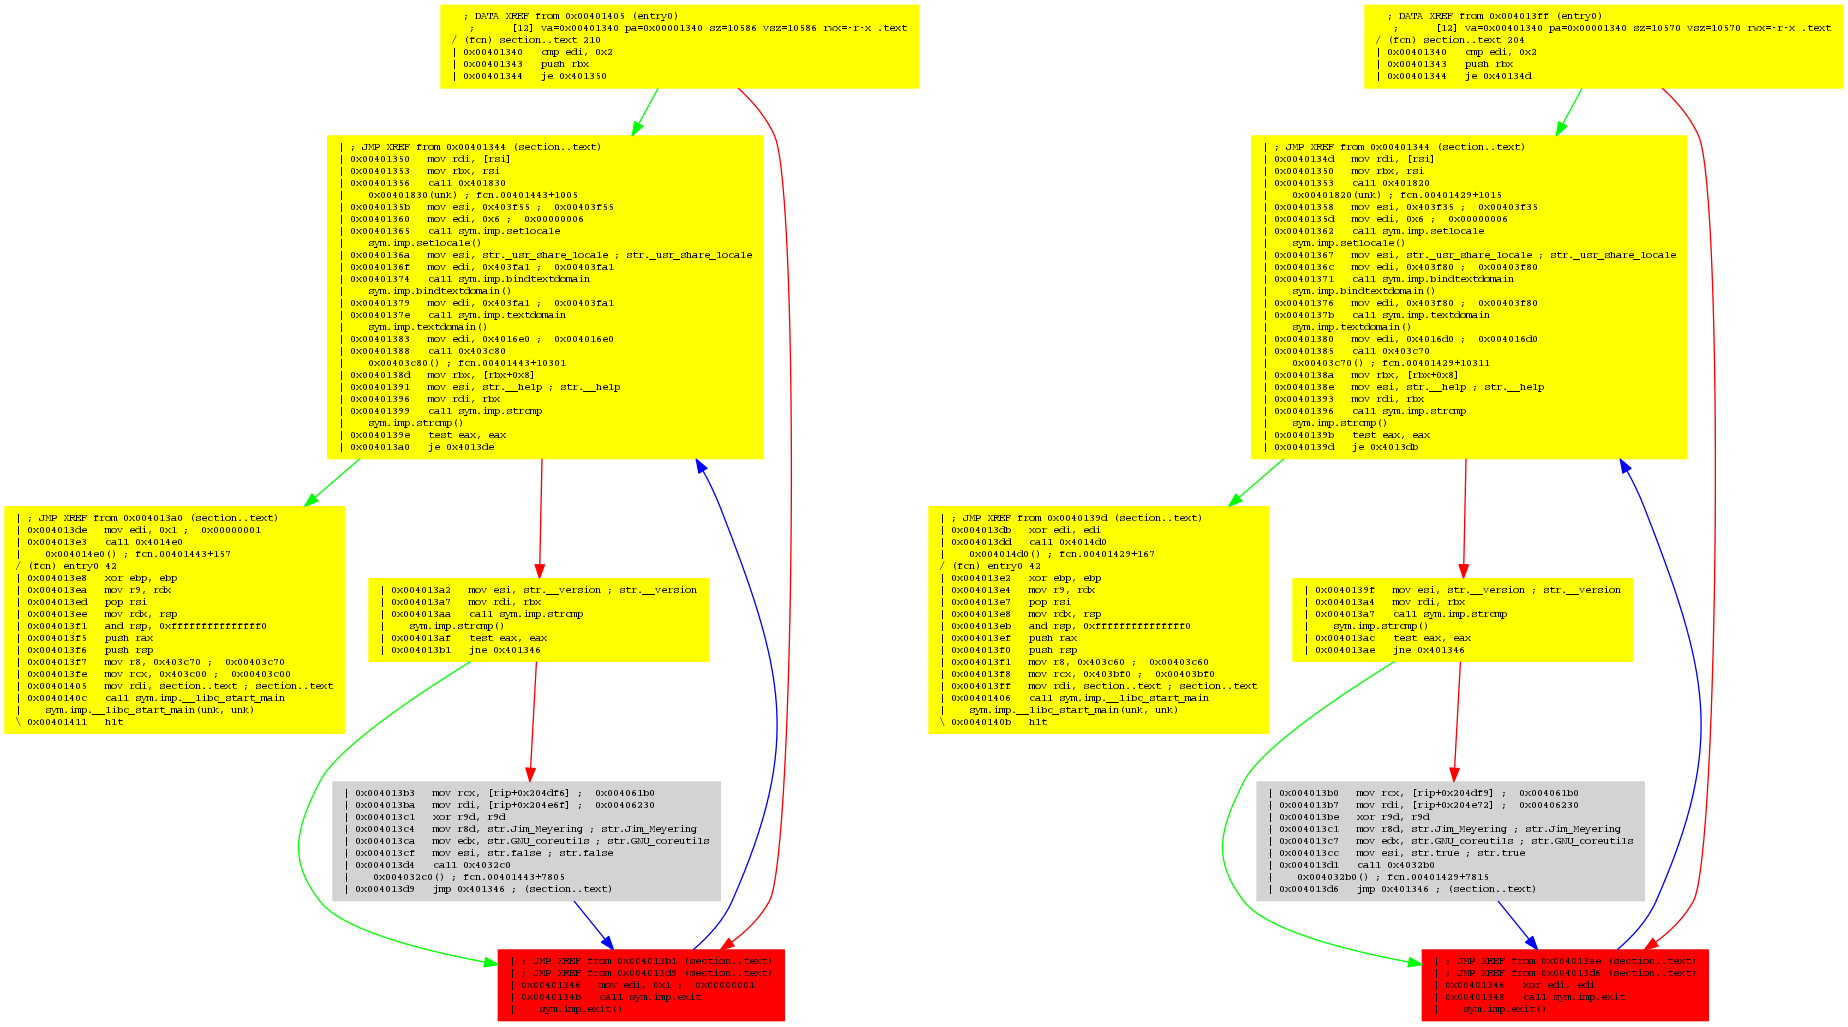
\includegraphics[width=\textwidth]{radiff2.png}
  \end{figure}
\end{frame}

\begin{frame}[fragile]
  \frametitle{Utilities}
     \begin{itemize}
        \item rax2
        \item rabin2
        \item rasm2
        \item radiff2
        \item \alert{rafind2}
        \item rahash2
        \item radare2
        \item rarun2
        \item ragg2/ragg2-cc
      \end{itemize}
\end{frame}

\begin{frame}[fragile]
  \center\textbf{rafind2} — Advanced commandline hexadecimal editor
  \noindent\makebox[\linewidth]{\rule{\paperwidth}{0.4pt}}
  \frametitle{Utilities: rafind2}
  \begin{verbatim}$ rafind2 -X -s passwd dump.bin\end{verbatim}
  \alert{Search for the string passwd}

\end{frame}

\begin{frame}[fragile]
  \frametitle{Utilities}
     \begin{itemize}
        \item rax2
        \item rabin2
        \item rasm2
        \item radiff2
        \item rafind2
        \item \alert{rahash2}
        \item radare2
        \item rarun2
        \item ragg2/ragg2-cc
      \end{itemize}
\end{frame}

\begin{frame}[fragile]
  \center\textbf{rahash2} — block based hashing utility
  \noindent\makebox[\linewidth]{\rule{\paperwidth}{0.4pt}}
  \frametitle{Utilities: rahash2}
  \begin{verbatim}$ rahash2 -a all binary.exe\end{verbatim}
  \alert{Display hashes of the whole file with all algos}
  \begin{verbatim}$ rahash2 -B -b 512 -a md5\end{verbatim}
  \alert{Compute md5 per block of 512}
  \begin{verbatim}$ rahash2 -B -b 512 -a entropy\end{verbatim}
  \alert{Compute md5 per block of 512}
  \begin{verbatim}$ echo -n "admin" | rahash2 -a md5 -s "\end{verbatim}
  \alert{Compute md5 of the string admin}

\end{frame}

\begin{frame}[fragile]
  \frametitle{Utilities}
     \begin{itemize}
        \item rax2
        \item rabin2
        \item rasm2
        \item radiff2
        \item rafind2
        \item rahash2
        \item \alert{radare2}
        \item rarun2
        \item ragg2/ragg2-cc
      \end{itemize}
\end{frame}

\section{Radare2 — Command line}

\begin{frame}[fragile]
  \frametitle{1 command <—> 1 Reverse-Engineering'notion}
  Keep in mind that:
  \begin{enumerate}
  \item Every character has a meaning i.e \alert{(w = write, p = print)}
  \item Every command is a succession of character i.e \alert{pdf = p <-> print d <-> disassemble f <-> function }
  \item Every command is documented with \textbf{cmd?}, i.e \alert{pdf?},\alert{?}, \alert{???}, \alert{???}, \alert{?\$?}, \alert{?@?}
  \end{enumerate}
\end{frame}

\begin{frame}[fragile]
  \frametitle{The \# command — hashing command}
  \begin{enumerate}
  \item Open a file with radare2 \alert{radare2 file.exe}
  \item Get Usage on the command \alert{\#?} \textbf{Usage: \#algo <size> @ addr}
  \item List of all existing algorithms \alert{\#\#}
  \item SHA1 \alert{\#sha1}
  \item Hashing from the begin \alert{\#sha1 @ 0}
  \item with a hash block size corresponding to the size of the file \alert{\#sha1 \$s @ 0x0}
 \end{enumerate}
This command is same as rahash2 -a sha1 file.exe
\end{frame}

\begin{frame}[fragile]
  \frametitle{The i command — information command}
  \begin{enumerate}
  \item Get Usage on the command \alert{i?}
  \item Same as \alert{rabin2}
  \item izj for displaying in json
  \item internal commands: \~, ls, \{\}, ..
 \end{enumerate}
\end{frame}

\begin{frame}[fragile]
  \frametitle{Radare2 — 'Major' command example: pf}
  Quick Demo
\end{frame}

\begin{frame}[fragile]
  \frametitle{Radare2 — CLI Main commands}
  \begin{enumerate}
   \item r2 -A or r2 then aaa : Analysis
   \item s : Seek
   \item pdf : Print disassemble function
   \item af? : Analyse function
   \item ax? : Analyse XREF
   \item /? : Search
   \item ps? : Print strings
   \item C? : Comments
   \item w? : Write
 \end{enumerate}
\end{frame}

\section{Radare2 — Visual mode}
\begin{frame}[fragile]
  \frametitle{Radare2 — Visual mode Main commands}
  \begin{enumerate}
  \item V? : Visual help
  \item p/P : rotate print modes
  \item move using arrows/hjkl
  \item o : seek to
  \item e : r2configurator
  \item v : Function list
  \item \_ : HUD
  \item V : ASCII Graph
 \end{enumerate}
\end{frame}

\section{Radare2 — WebUI}
\begin{frame}[fragile]
  \frametitle{Radare2 — WebUI}
  r2 -A -c=H filename
    \begin{figure}
  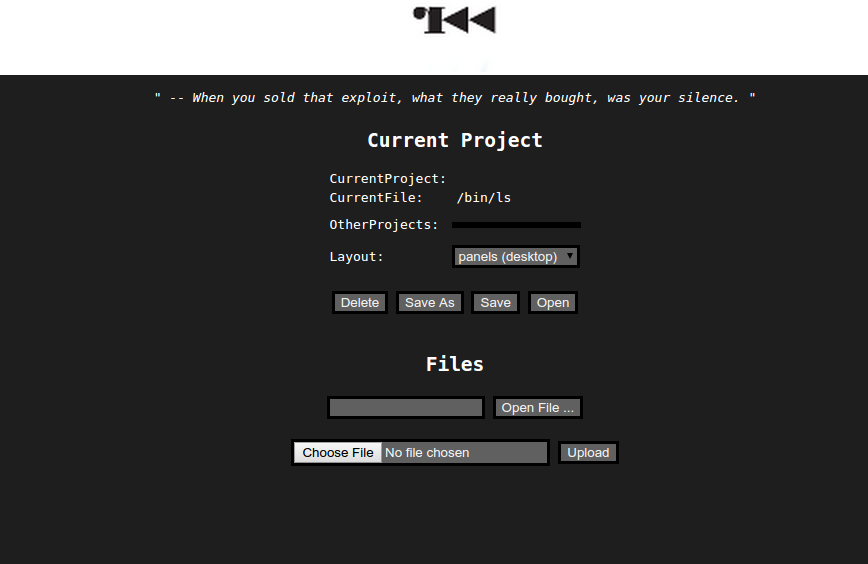
\includegraphics[width=\textwidth]{web.png}
  \end{figure}
\end{frame}

\section{Radare2 — Debugger}

\begin{frame}[fragile]
  \frametitle{Radare2 — Debugger}
  \begin{enumerate}
  \item radare2 -d
  \item Quickly switch to Visual debugger mode: Vpp
  \item OllyDBG/IDApro shortcuts friendly
 \end{enumerate}
\end{frame}

\begin{frame}[fragile]
  \frametitle{Utilities}
     \begin{itemize}
        \item rax2
        \item rabin2
        \item rasm2
        \item radiff2
        \item rafind2
        \item rahash2
        \item radare2
        \item \alert{rarun2}
        \item ragg2/ragg2-cc
      \end{itemize}
\end{frame}

\begin{frame}[fragile]
  \frametitle{Rarun2}
  \center\textbf{Rarun2} — run programs in exotic environments
  \noindent\makebox[\linewidth]{\rule{\paperwidth}{0.4pt}}
  \begin{enumerate}
  \item Environnment setup tools for radare2
  \item most useful with debugger
  \item aslr, stdout, arguments, r2preload ...
 \end{enumerate}
\end{frame}

\begin{frame}[fragile]
  \frametitle{Utilities}
     \begin{itemize}
        \item rax2
        \item rabin2
        \item rasm2
        \item radiff2
        \item rafind2
        \item rahash2
        \item radare2
        \item rarun2
        \item \alert{ragg2/ragg2-cc}
      \end{itemize}
\end{frame}

\begin{frame}[fragile]
  \frametitle{Ragg2/Ragg2-cc}
  \center\textbf{Ragg2/Ragg2-cc} — frontend for compiling shellcodes
  \noindent\makebox[\linewidth]{\rule{\paperwidth}{0.4pt}}
\end{frame}

\begin{frame}[fragile]
  \frametitle{Now your turn!}
    \begin{itemize}
    \item \alert{Crackmes:} IOLI-Crackme, flare-on 2015 challenges
    \item \alert{Exploitation:} pwn1, pwn2, ropasaurus
    \item \alert{Malware(1/3):} Practical malware analysis samples
    \item \alert{Malware(2/3):} Any RAT samples see decoder on: TODO
    \item \alert{Malware(3/3):} AVCaesar.lu, MalekalDB, TODO
    \item \alert{Firmware/BIOS/UEFI:} TODO
    \end{itemize}
\end{frame}

\begin{frame}[fragile]
  \frametitle{Documentation}
    \begin{itemize}
    \item \alert{Website:} http://rada.re/
    \item \alert{Blog:} http://radare.today
    \item \alert{Book:} http://maijin.gitbooks.io/radare2book/content/
    \end{itemize}
\end{frame}

\section{Exploitation (jvoisin work :-) )}

\begin{frame}[fragile]
	\begin{center}
		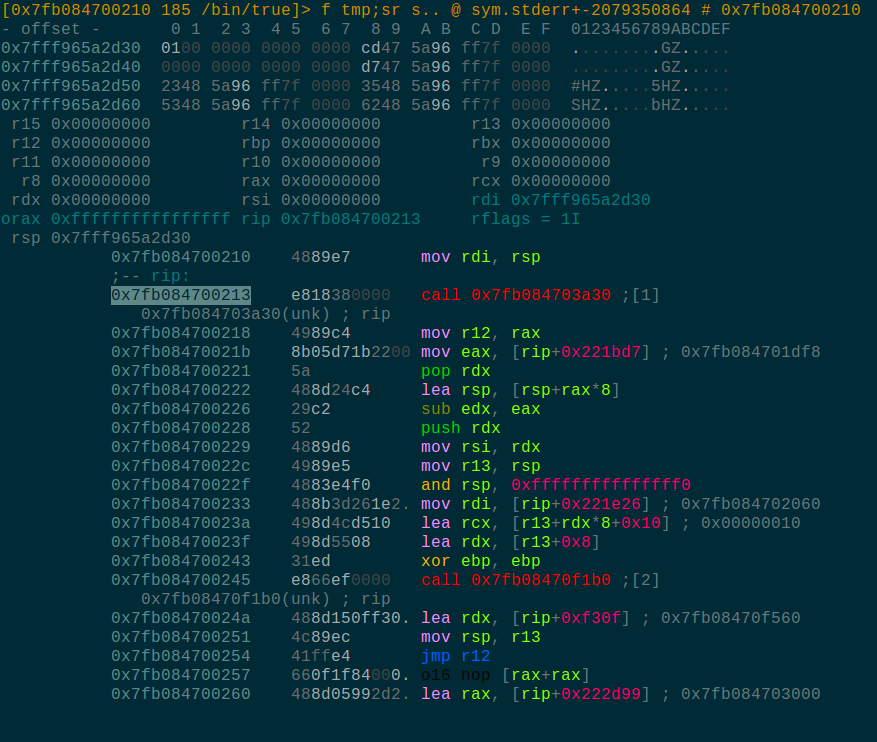
\includegraphics[width=\textwidth]{regstacklisting.png}
	\end{center}
\end{frame}

\begin{frame}{Stack}
	\begin{center}
	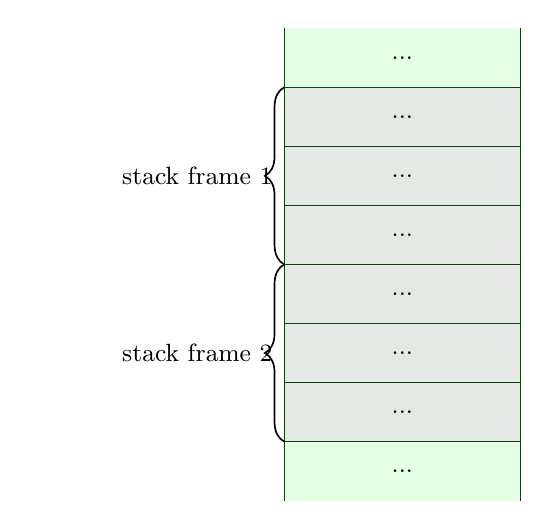
\begin{tikzpicture}[scale=0.75]
		\small
		\stacktop{}
		\startframe
		\padding{1}{...}
		\padding{1}{...}
		\padding{1}{...}
		\finishframe{stack frame 1}
		\startframe
		\padding{1}{...}
		\padding{1}{...}
		\padding{1}{...}
		\finishframe{stack frame 2}
		\stackbottom{}
	\end{tikzpicture}
	\end{center}
\end{frame}

\begin{frame}{Stack smashing}
	\begin{center}
		\begin{columns}
			\begin{column}{.5\textwidth}
				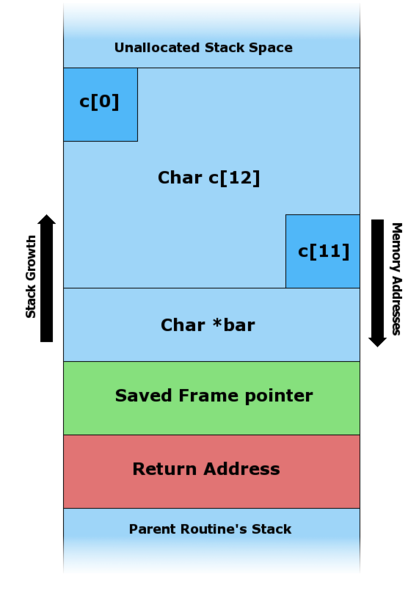
\includegraphics[height=6.5cm]{overflow1.png}
			\end{column}
			\begin{column}{.5\textwidth}
				\only<1>{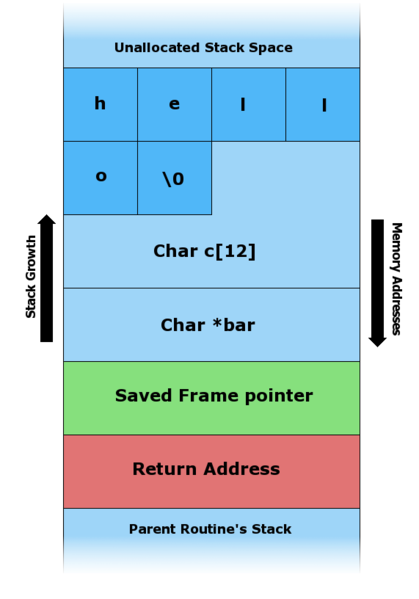
\includegraphics[height=6.5cm]{overflow2.png}}
				\only<2>{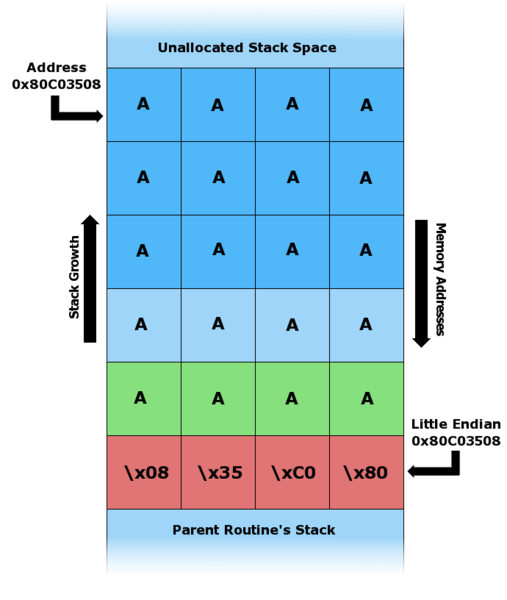
\includegraphics[height=6.5cm]{overflow3.png}}
			\end{column}
		\end{columns}
	\end{center}
\end{frame}

\section{Pwn1}
\begin{frame}{Pwn1}
	\begin{itemize}
		\item Written for this workshop
		\item Oldschool \emph{classic} example
		\item You'll write the final exploit
	\end{itemize}
\end{frame}

\begin{frame}{Hu-ho.}
	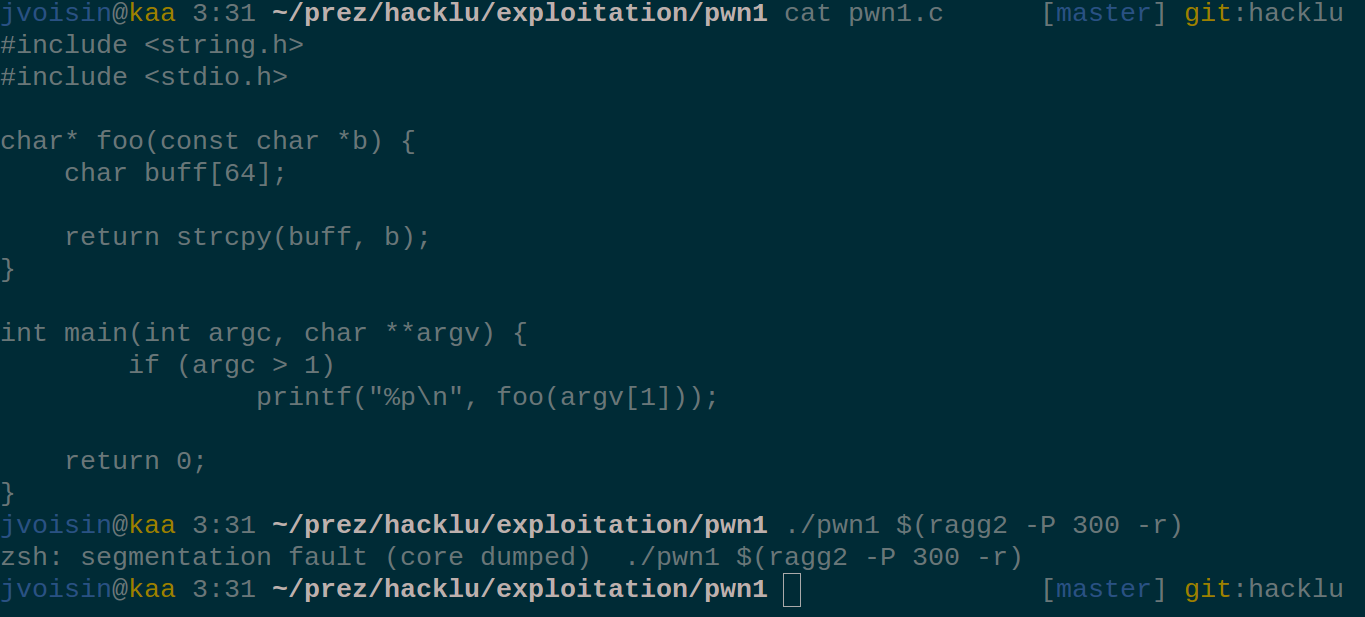
\includegraphics[width=\textwidth,height=6.5cm]{segfault_pwn1.png}
\end{frame}

% Explain what a De Bruijn pattern is
\begin{frame}{De Bruijn patterns}
	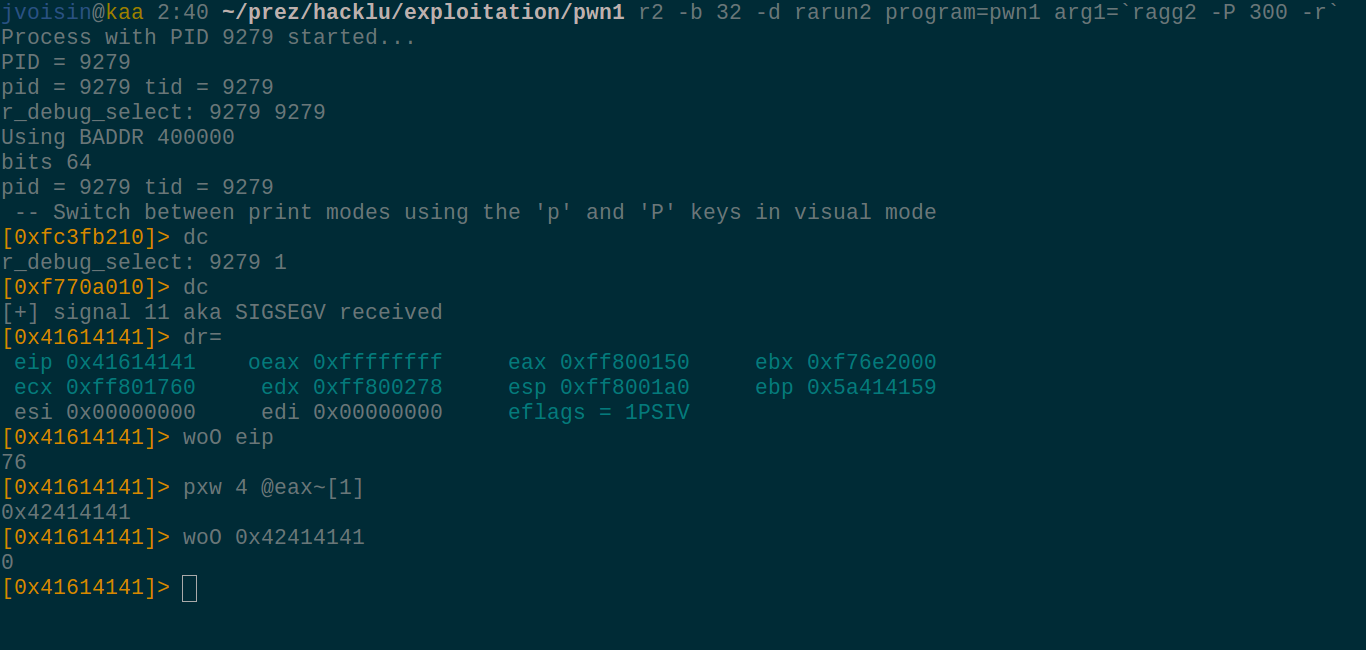
\includegraphics[width=\textwidth,height=6.5cm]{bruijn.png}
\end{frame}

\begin{frame}{Exploit!}
	\begin{columns}
		\begin{column}{.3\textwidth}
			\begin{itemize}
				\item No ALSR
				\item No NX
				\item No Canary
			\end{itemize}
		\end{column}
		\begin{column}{.7\textwidth}
			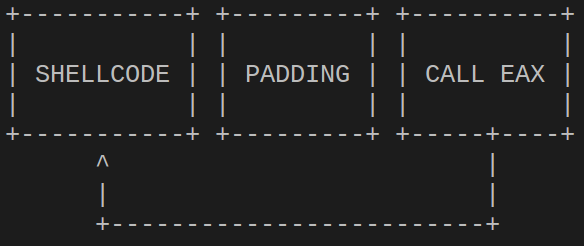
\includegraphics[width=\textwidth,height=2cm]{pwn1_shellcode.png}
		\end{column}
	\end{columns}
\end{frame}

\begin{frame}{Generate shellcode}
	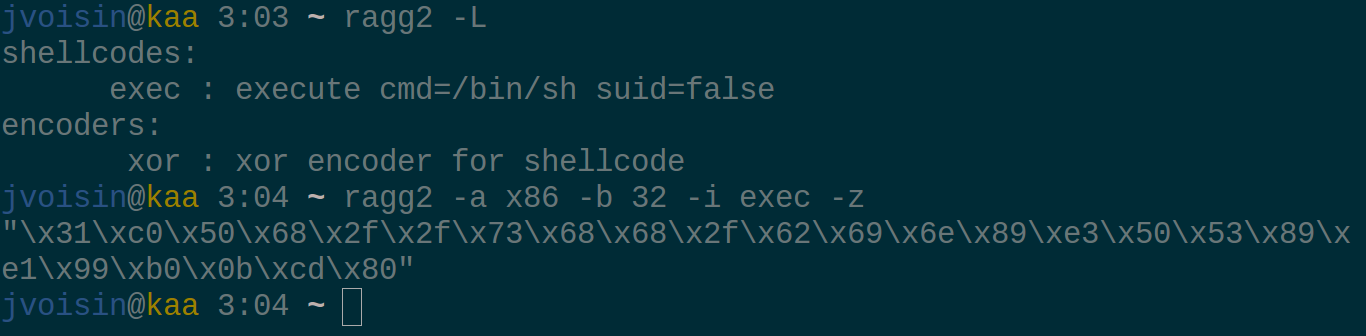
\includegraphics[width=\textwidth]{binsh.png}
	\vskip.5cm
	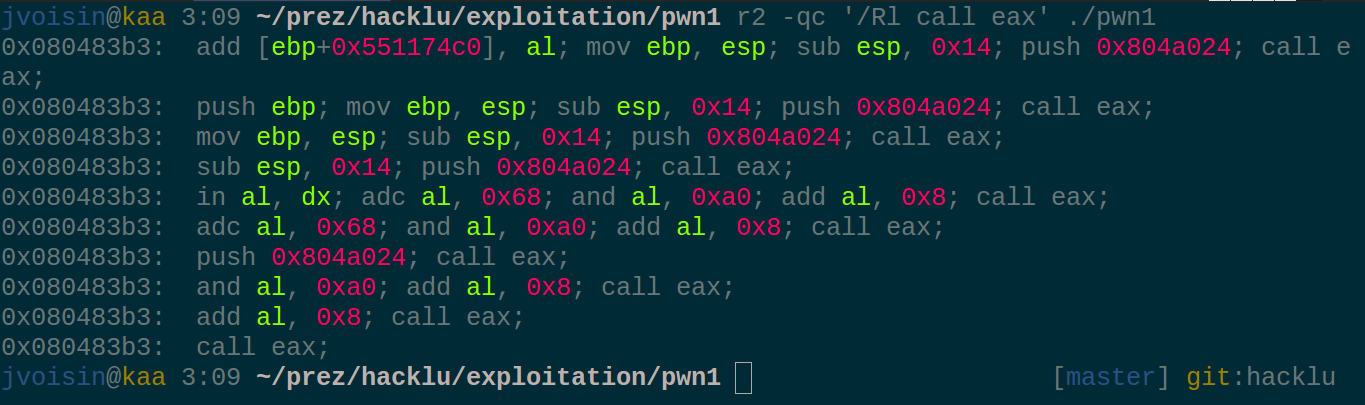
\includegraphics[width=\textwidth]{rop_pwn1.png}
\end{frame}

\begin{frame}{Your turn!}
	\begin{center}
		Write a working exploit!
	\end{center}
\end{frame}

\begin{frame}{Show me yours, I'll show you mine}
	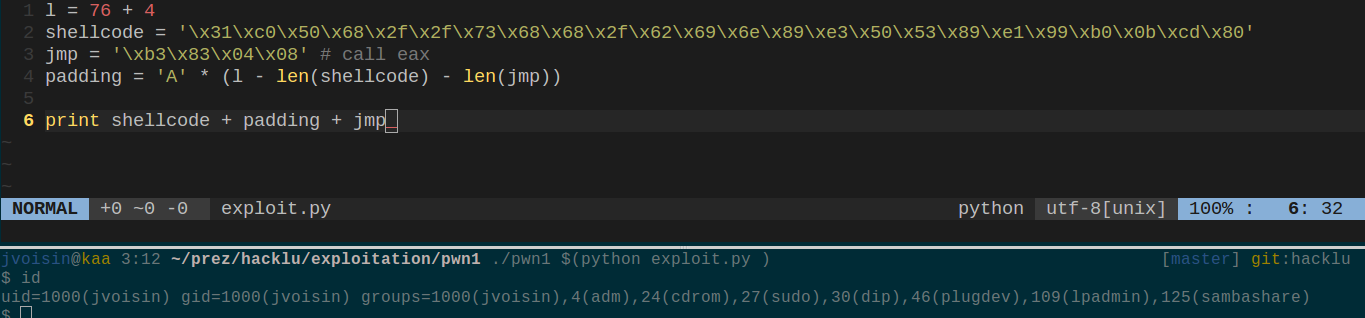
\includegraphics[width=1.05\textwidth,height=4.5cm]{exploit_pwn1.png}
\end{frame}

\section{Malware Analysis}

\begin{frame}[fragile]
  \frametitle{Other r2 commands I use frequently at work}
  \begin{enumerate}
   \item \#?
   \item ?d, i?
   \item Visual mode and associated (VVV, Vv, ;, ...)
   \item Analysis command (axt, agf, ...)
   \item /m?, /C?, pf, px?, p6d, p=
   \item yara, zF
   \item pr, wt
   \item basic zsh/bash scripting, r2-pipe
 \end{enumerate}
\end{frame}

\begin{frame}[fragile]
  \frametitle{Documentation}
    \begin{itemize}
    \item \alert{Website:} http://rada.re/
    \item \alert{Blog:} http://radare.today
    \item \alert{Book:} http://maijin.gitbooks.io/radare2book/content/
    \end{itemize}
\end{frame}

\end{document}
